\section{Error budget}
\label{sec:budget}

\subsection{A sufficient condition}

For a protected evaluation $(R,t)$ with non-empty support let the margin be
$m_R(t) = |f_R(X)(t) - \theta|$ and let $L_R(t)$ be a Lipschitz constant of
$F$ on $\mathbb{R}^{|S_R(t)|}$ in the sup norm. \code{last},
\code{avg\_over\_time}, \code{min\_over\_time} and \code{max\_over\_time} have
$L = 1$; \code{sum\_over\_time} has $L = |S_R(t)|$. The tolerance of the
evaluation is $\tau_R(t) = m_R(t)/L_R(t)$ and the budget of sample $i$ is
the minimum over every evaluation that reads it:
\begin{equation}
  \eps_i = \min\{\tau_R(t) : R \in \R,\ t \in P_R,\ i \in S_R(t)\},
  \qquad \min\emptyset = +\infty .
  \label{eq:budget}
\end{equation}

The condition is $f_R(X)(t) \bowtie \theta$ or its negation, so on the
original data it is one of $f > \theta$, $f \ge \theta$, $f < \theta$,
$f \le \theta$. Two properties of this inequality matter below.

\begin{definition}[Tight, upper and lower evaluations]
\label{def:tight}
A protected evaluation $(R,t)$ is \emph{tight} if the inequality that holds
on $X$ is strict, i.e.\ $c_R(X)(t) = 1$ with ${\bowtie} \in \{>,<\}$, or
$c_R(X)(t) = 0$ with ${\bowtie} \in \{\ge,\le\}$. Then a reconstruction with
$f_R(Y)(t) = \theta$ already flips the condition, so the error must stay
strictly below the tolerance. It is \emph{upper} if $f_R(X)(t)$ lies on
the side of $\theta$ that only a decrease of the aggregate can leave
($c_R(X)(t) = 1$ with ${\bowtie} \in \{>,\ge\}$, or $c_R(X)(t) = 0$ with
${\bowtie} \in \{<,\le\}$), and \emph{lower} otherwise.
\end{definition}

We call the set of reconstructions
$\{Y : |y_i - x_i| \le \eps_i \text{ for all } i \in I\}$ the
\emph{box budget}: it bounds every error symmetrically.

\begin{theorem}[Box budget]
\label{thm:budget}
If $|y_i - x_i| \le \eps_i$ for all $i$, strictly on the supports of tight
evaluations, then $c_R(Y)(t) = c_R(X)(t)$ for all
$R \in \R$ and $t \in P_R$, and hence $D_R(Y) = D_R(X)$ on every grid (on $T$
for \code{rate}).
\end{theorem}
\begin{proof}
Supports depend on timestamps only. By the Lipschitz bound
$|f_R(Y)(t) - f_R(X)(t)| \le L_R(t)\max_{i\in S_R(t)}|e_i| \le m_R(t)$,
strictly when tight, so $f_R(Y)(t)$ stays on the same side of $\theta$.
\Cref{lem:phase,lem:automaton} finish the proof.
\end{proof}

The Lipschitz step is ordinary quantity-of-interest error
propagation~\cite{jiao2022qoi}. What is specific is the granularity: errors
live on samples and margins on evaluations, and one sample feeds every
evaluation whose window contains it, so the budget is a minimum over
overlapping windows. Two consequences follow. A streaming encoder needs a
lookahead of the longest window $\max_R w_R$, so the natural deployment point
is block compaction (Prometheus compacts 2-hour blocks) or a buffered proxy.
And a sample at margin zero must be exact. Since any smaller budget is also
sufficient, a pointwise cap $\min(\eps_i, \eps_{\max})$ adds a fidelity
guarantee for dashboards without weakening the alert guarantee.

\subsection{One-sided budget}

The box budget of \cref{thm:budget} is pessimistic: near a threshold a series
mostly lies on one side, and only errors towards $\theta$ can flip a
decision.

\begin{corollary}[One-sided budget]
\label{cor:onesided}
Let $\delta^-_i$ (the \emph{downward} budget) be the minimum of
$\tau_R(t)$ over the upper evaluations whose support contains $i$, and
$\delta^+_i$ (the \emph{upward} budget) the same minimum over the lower
ones, with $\min\emptyset = +\infty$ (\cref{def:tight}). If
$-\delta^-_i \le y_i - x_i \le \delta^+_i$ for all $i$ (strict where
tight), every protected condition is preserved.
\end{corollary}
\begin{proof}
All aggregates above are non-decreasing in each argument. For an upper
$(R,t)$ let $z_i = \min(y_i, x_i)$ on its support. Then
$|z_i - x_i| \le \delta^-_i \le \tau_R(t)$, so $z$ satisfies
\cref{thm:budget} at $(R,t)$, and $F(y) \ge F(z)$ keeps $f_R(Y)(t)$ on the
upper side. Lower evaluations are symmetric with $\max$.
\end{proof}

Since $\eps_i = \min(\delta^-_i, \delta^+_i)$, the box budget is contained in the
one-sided set, and the difference is large: a sample read only by upper
evaluations may move up without limit (\cref{fig:budget}). The coder exploits it only if it can
place reconstructions asymmetrically (\cref{sec:codec}); the ablation shows
that the one-sided budget alone, with round-to-nearest, gains little
(\cref{sec:ablation}).

\begin{figure}[t]
\centering
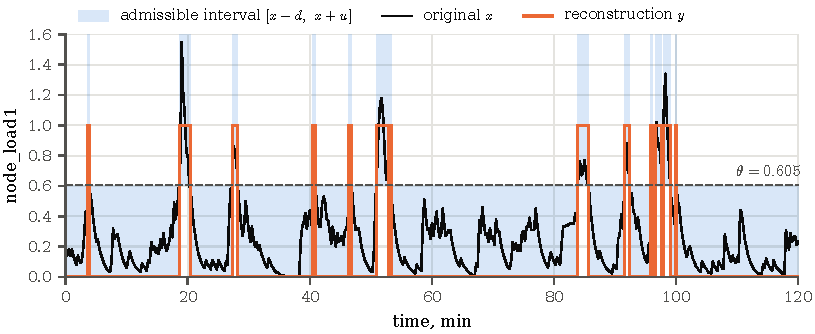
\includegraphics[width=\linewidth]{budget}
\caption{One-sided budget and the codec's reconstruction on two hours of
\code{node\_load1} (7-day snapshot, rule \code{last > }$\theta$ with $\theta$
at the 95th percentile). Below $\theta$ only the upward error is bounded,
above it only the downward one, so the admissible interval (shaded) is a
half-line and the reconstruction collapses to two levels; every alert
decision is unchanged.}
\label{fig:budget}
\end{figure}

\subsection{Counters and \code{rate}}
\label{sec:budget-rate}

We restate Prometheus' \code{rate} (\code{extrapolatedRate} in
\code{promql/functions.go}~\cite{promsrc}) for one evaluation $(R,t)$ with
$|S_R(t)| \ge 2$. Let $f$ and $l$ be the first and last indices of the
support $S_R(t)$. The rule reads:
\begin{itemize}
  \item the \emph{increase}
    $\Delta = x_l - x_f + \rho$, where
    $\rho = \sum_{i \in S_R(t),\, i > f,\, x_i < x_{i-1}} x_{i-1}$ adds back
    the value lost at every reset inside the window;
  \item the \emph{sampled interval} $\sigma = s_l - s_f$, the time covered
    by the samples;
  \item the \emph{extrapolation distances} $h_{\mathrm{s}}$ and
    $h_{\mathrm{e}}$ from the first and last sample to the window's start
    $t - w$ and end $t$, each replaced by half the mean sample spacing
    when it reaches $1.1$ times that spacing; they depend on timestamps
    only;
  \item the \emph{zero distance} $h_0 = \sigma x_f / \Delta$, the time
    before $s_f$ at which a counter growing at the window's average speed
    was zero (used only when $\Delta > 0$).
\end{itemize}
The increase is extrapolated to the window boundaries, but not past the
counter's zero point, and divided by the range in seconds:
\[
  \mathrm{rate} = \frac{\Delta}{w}\cdot
  \frac{\sigma + \min(h_{\mathrm{s}}, h_0) + h_{\mathrm{e}}}{\sigma}.
\]

\begin{proposition}
\label{prop:rate}
(a) The reset indicator $[x_i < x_{i-1}]$ is a comparison of two samples, so
an arbitrarily small error can create a reset and change $\Delta$ by a whole
counter value; no positive symmetric budget preserves \code{rate} in general.
(b) The closed-loop floor quantizer
$y_i = y_{i-1} + q\lfloor (x_i - y_{i-1})/q\rfloor$ (exact when the step
count would be negative) gives $x_i - q < y_i \le x_i$ and preserves
$x_i \ge x_{i-1} \Rightarrow y_i \ge y_{i-1}$; keeping the two samples
around each true reset exact preserves the reset set.
(c) On the reset-preserving set, $\mathrm{rate}$ is Lipschitz in
$(\Delta, x_f)$ away from $x_f = 0$, with constant
$\approx (2 + r)/w$ for a densely sampled window with $r$ resets.
(d) Under (b), $\Delta$ and $x_f$ read only the window's first and last
samples and the preserved reset values, so the budget of a \code{rate}
evaluation applies to the two ends of its window only.
\end{proposition}

The implementation does not use the constant in (c): it computes a sound
interval enclosure of the \code{rate} formula over the box
$y_i \in [x_i - \eps, x_i]$, including the zero-point branch, and finds the
largest safe $\eps$ by bisection. By (d), with a 30\,s evaluation grid on
15\,s scrapes about half of a counter's samples are no window's end and are
constrained only by monotonicity.

\subsection{Where no budget exists}

A positive budget exists at $x$ iff $x$ is interior to the set of inputs
with the same condition. Equality tests, \code{changes()}, \code{floor} and
\code{round} inside expressions, and label-selecting aggregations
(\code{topk}) violate this at their decision points and need exact samples
there; ratios and \code{histogram\_quantile} are locally Lipschitz and need
an interval enclosure like \code{rate}.

\subsection{Floating point and complexity}

The budget is computed in floating point. The code subtracts a rounding
slack from the margin: a floating-point sum of $n$ terms has error at most
$\gamma_{n-1}\sum_i|v_i|$ with $\gamma_n = nu/(1 - nu)$ and unit roundoff
$u = 2^{-53}$~\cite{higham2002accuracy}.
The code also uses the next representable value below the tolerance for strict
comparisons. Monotonicity holds bitwise for \code{last}, \code{min} and
\code{max}; Prometheus sums with Kahan compensation, which is not monotone,
so for \code{sum/avg} \cref{cor:onesided} goes through the error bound
instead, and an evaluation whose margin is within the rounding slack is
constrained in both directions.

Supports are monotone in $t$, so all supports follow by two pointers, window
aggregates by a two-stacks sliding queue, and the per-sample minimum in
\eqref{eq:budget} is a sliding minimum over instants (monotone deque). The
budget costs $O(n + |P_R|)$ per rule; \code{rate} adds a bisection of about
a dozen enclosure evaluations per instant.
